\documentclass{beamer}
\usepackage{fancybox}
\usepackage{tikz}
\usetikzlibrary{arrows.meta,
                chains,
                positioning, 
                shadows.blur, shapes.arrows}
              
\usetheme{Madrid}

\title{Neuro-symbolic AI}
\author{Robert Hoehndorf}
\date{\today}

\begin{document}

\frame{\titlepage}

\begin{frame}
\frametitle{Overview}
\begin{itemize}
\item AI:
  \begin{itemize}
  \item Statistical
  \item Neural
  \item Symbolic
  \end{itemize}
\end{itemize}
\end{frame}

\begin{frame}
  \frametitle{Outline}
  \begin{itemize}
  \item Introduction
  \item Fuzzy Logic and Logic Tensor Networks, LNNs
  \item Knowledge graphs, Question/Query answering
  \item Logic Programming
    \begin{itemize}
    \item ProbLog, ASP
    \item ILP
    \end{itemize}
  \item Markov Logic
  \item Geometric and algebraic methods, model theory
  \end{itemize}
\end{frame}

\begin{frame}
  \frametitle{Format and Evaluation}
  \begin{itemize}
  \item seminar-style course
    \begin{itemize}
    \item reading 2-3 research papers per week
    \item presentation (20\%) and discussion (20\%)
    \end{itemize}
  \item research project (60\%)
    \begin{itemize}
    \item start within the first 3 weeks
    \item individual project
    \item frequent project presentations/updates
    \item research paper
    \end{itemize}
  \end{itemize}
\end{frame}

\begin{frame}
  \frametitle{Research project}
  \begin{itemize}
  \item must combine neural/statistical and symbolic methods
  \item focus on either novel method or application
  \item aim at end of the course: research paper
    \begin{itemize}
    \item may be submitted to conference or journal
    \end{itemize}
  \end{itemize}
\end{frame}

\begin{frame}
  \frametitle{What is a viable research question?}
  \begin{itemize}
  \item qualitative (proof) vs quantitative (experiment)
  \item usually: improve method $X$ to address limitation $Y$
    \begin{itemize}
    \item $X$ --- existing method to solve some problem
    \item $Y$ --- how to find?
      \begin{itemize}
      \item analysis (primary research!)
      \item theoretical argument
      \item literature (check Discussion for limitations)
      \end{itemize}
    \end{itemize}
  \item or: develop method $X$ to overcome limitation $Y$ in methods
    addressing problem $Z$
  \end{itemize}
\end{frame}

\begin{frame}
  \frametitle{Examples}
  \begin{itemize}
  \item Can we develop an algorithm with $O(n \cdot \log{n})$ runtime
    that sorts a list of integers accurately in descending order?
    \pause
  \item Can graph neural networks improve reasoning over first order
    theories?
    \pause
    \begin{itemize}
    \item These are not good research question on their own!
    \item How are current methods limited?
    \item How could GNNs overcome this limitation?
      \begin{itemize}
      \item Not: ``Apply X to Y'' but ``X can solve limitation Z in
        algorithms for Y''
      \end{itemize}
    \end{itemize}
  \end{itemize}
\end{frame}

\begin{frame}
  \frametitle{Answering the question}
  \begin{itemize}
  \item baseline
    \begin{itemize}
    \item how does method $X'$ solve problem $P$ now?
    \item quantify, and justify: which measure is appropriate? which
      test case / dataset is appropriate?
    \item are there different {\bf types} of methods to solve $P$? Did
      you include a representative for each?
    \item Why did you include method $X'$ over $X''$?
    \end{itemize}
    \pause
  \item workflow $W$: build a skeleton method to solve problem $P$
    \begin{itemize}
    \item can you reuse existing code? Check Github...
    \item you need to get from input (your dataset) to output (a
      number --- quantify!)
    \end{itemize}
    \pause
  \item actual methods research
    \begin{itemize}
    \item add your idea to $W$ and quantify --- do performance metrics
      improve?
    \item one idea at a time, quantify, iterate
    \item tune, optimize (usually not part of the RQ)
    \end{itemize}
  \end{itemize}
\end{frame}

\begin{frame}
  \frametitle{Considerations}
  \begin{itemize}
  \item feasibility: workplan/idea adequate to answer the question?
  \item novel: did somebody try before? How is your work different
    from others?
    \begin{itemize}
    \item find limitation in state of the art --- from experience,
      papers, etc.
    \item know novel, emerging methods deeply --- know their
      limitations, which problems they can solve and how
    \item then: apply novel method to problem to overcome limitation
    \end{itemize}
    \pause
  \item interesting and relevant: will people care? Can you explain
    why its relevant, important? For whom? Can others build on your
    results, use your method?
    \begin{itemize}
    \item impact
    \item problem statement
    \end{itemize}
  \end{itemize}
\end{frame}

\begin{frame}
  \frametitle{Project evaluation}
  \begin{enumerate}
  \item clear description of problem to be solved (10\%)
  \item description and analysis of state of the art (10\%)
    \begin{itemize}
    \item how is the state of the art limited?
    \end{itemize}
  \item method to overcome limitation of the state of the art (20\%)
    \begin{itemize}
    \item must combine neural/statistical and symbolic methods!
    \end{itemize}
  \item experiments or proof (10\%)
  \item manuscript, report, paper (10\%)
    \begin{itemize}
    \item this report will be used for evaluation (and presentations)
    \end{itemize}
  \end{enumerate}
\end{frame}

% Motivation
\begin{frame}
\frametitle{Motivation}
\begin{itemize}
\item Growing interest in combining Machine Learning with Knowledge
  Representation
\item Motivated by complementary functionalities and strengths
\item Fueled by recent keynotes and workshops in the field
\end{itemize}
\end{frame}

\begin{frame}
  \frametitle{What is Artificial Intelligence?}
  \begin{quote}
    Why is there so much excitement about neural networks today, and
    how is this related to research in AI? Much has been said, in
    the popular press [...]
  \end{quote}
  \pause
  (Marvin Minsky, 1991)
  \pause
  \begin{block}{Symbolic AI (GOFAI)}
    A physical symbol system takes physical patterns (symbols),
    combines them into structures (expressions) and manipulates them
    (using processes) to produce new expressions.
  \end{block}
\end{frame}

% Two Families of Techniques
\begin{frame}
\frametitle{Two Families of Techniques}
\begin{itemize}
\item Learning Methods: Predominantly statistical
\item Reasoning Methods: Predominantly discrete
\item General conclusion: Human-level AI requires symbiotic
  collaboration of data and models
\end{itemize}
\end{frame}

\begin{frame}
\frametitle{Why symbols?}
\begin{itemize}
\item Symbols are physical entities that can encode for our {\em
    knowledge} of the world (e.g., for a proposition $P$)
\item We want knowledge to affect our decisions:
  \begin{itemize}
  \item do A if world believed to satisfy P
  \end{itemize}
\item $P$ may not be {\em explicitly} represented $\Rightarrow$ need
  symbol manipulation and search
\item Example:
  \begin{itemize}
  \item Patient $x$ is allergic to medication $m$: $all(x,m)$
  \item Anybody allergic to $m$ is also allergic to $m'$: $\forall
    y(all(y,m) \rightarrow all(y,m'))$
  \item It's not safe to prescribe medication if allergic: $\forall a,
    b (all(a,b) \rightarrow \neg safe(a,b))$
  \item Is it safe to prescribe $m'$ to $x$: $safe(x, m')$ ?
  \end{itemize}
\item symbol systems: formal logic, arithmetic, algebra, term/graph
  rewriting systems, digital computer
\end{itemize}
\end{frame}

\begin{frame}
  \frametitle{Physical Symbol System Hypothesis}
  \begin{quote}
    A physical symbol system has
    the necessary and sufficient means for general intelligent
    action. [Newell \& Simon, 1976]
  \end{quote}
\end{frame}

\begin{frame}
  \frametitle{Limitations}
  \centerline{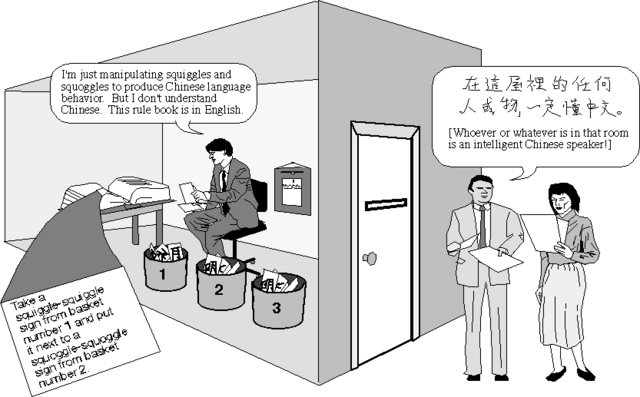
\includegraphics[width=.75\textwidth]{chinese-room.png}}  
  \begin{itemize}
  \item symbol grounding (hard to learn from data)
  \item very inflexible (inconsistencies, mathematical proofs)
  \item yet: sound and complete
  \end{itemize}
\end{frame}

\begin{frame}
  \frametitle{Connectionist systems}
  \begin{itemize}
  \item parallel distributed processing units, neural networks
  \item biologically inspired
  \item non-symbolic, sub-symbolic
    \begin{itemize}
    \item learn from data
    \end{itemize}
  \item challenges:
    \begin{itemize}
    \item interpretability
    \item compositionality
    \end{itemize}
  \item Research question: how much of intelligent behavior is
    symbolic?
  \item Research theme: how to combine symbolic and connectionist
    systems to overcome their individual limitations?
  \end{itemize}
\end{frame}

\begin{frame}
  \frametitle{Motivation}
  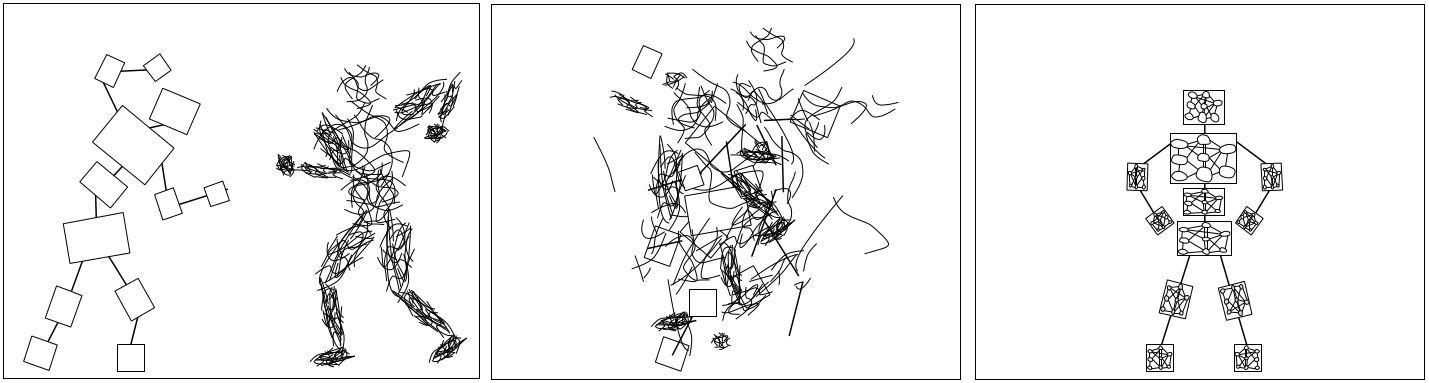
\includegraphics[width=\textwidth]{minsky-figure.png}
\end{frame}

\end{document}

% Introduction:

% Minsky's paper

% http://arxiv.org/abs/1905.12389

% http://arxiv.org/abs/2305.08876

% http://arxiv.org/abs/2302.02093




% From knowledge graph to knowledge base completion


% Neural logical query answering

%%% Local Variables:
%%% mode: latex
%%% coding: utf-8
%%% TeX-master: t
%%% eval: (TeX-run-style-hooks "beamer")
%%% End:
